\documentclass[ngerman]{scrartcl}
\usepackage{graphicx}
\usepackage{personal}
\usepackage{wrapfig}
\usepackage{booktabs}
\usepackage{subcaption}
\usepackage{listings}
\usepackage{parskip}
%\lstset{numbers=left, frame=tblr, basicstyle=\tiny, tabsize=3}
\definecolor{codegreen}{rgb}{0,0.6,0}
\definecolor{codegray}{rgb}{0.5,0.5,0.5}
\definecolor{codepurple}{rgb}{0.58,0,0.82}
\definecolor{backcolour}{rgb}{0.95,0.95,0.92}

\lstdefinestyle{mystyle}{
    backgroundcolor=\color{backcolour},   
    commentstyle=\color{codegreen},
    keywordstyle=\color{magenta},
    numberstyle=\tiny\color{codegray},
    stringstyle=\color{codepurple},
    basicstyle=\ttfamily\footnotesize,
    breakatwhitespace=false,         
    breaklines=true,                 
    captionpos=b,                    
    keepspaces=true,                 
    numbers=left,                    
    numbersep=5pt,                  
    showspaces=false,                
    showstringspaces=false,
    showtabs=false,                  
    tabsize=2
}
\lstset{style=mystyle}


\begin{document}
\begin{titlepage}
\begin{center}
    \vspace{15cm}
    \huge{Lab 2}\\
    \vspace{2cm}
    \Huge{AML}\\
    \vspace{2cm}
    \Large{Elia Faure-Rolland}\\
    \Large{Tarek Saade}\\
    \Large{Ana Martinez}\\
    \Large{Jonas Thalmeier}\\
    \vspace{1cm}
    19/05/2025
\end{center}
\vspace{3cm}
\begin{figure}[h]
    \centering
    
\includegraphics[width=.5\textwidth]{Figures/Eurecom.png}
\end{figure}
\end{titlepage}

%\newpage
%\tableofcontents
\thispagestyle{empty}
\newpage
\setcounter{page}{1}

\section*{Introduction}
In this project, we address the task of Anomalous Sound Detection by replicating a subset of the well-known DCASE challenge. Specifically, we focus on detecting anomalous sounds emitted by industrial machines, where early identification of mechanical failure can prevent costly downtimes. A key difficulty in this task is the scarcity and unpredictability of real-world anomalous data, which necessitates the use of unsupervised or semi-supervised methods trained solely on normal samples. Our objective is to develop a system that, given only normal sound recordings from a subset of machines, can classify whether an unseen audio recording is normal or anomalous. The dataset used in this work is derived from the official DCASE 2020 challenge and includes machine operating sounds from two major sources: ToyADMOS and the MIMII dataset. These recordings capture six types of machines, but for feasibility within the scope of the AML course, we concentrate solely on the Slide Rail machine type. The data consists of 10-second single-channel audio files, with anomalous versions generated by deliberately damaging machines and mixing them with background noise recorded in real factory environments. We work with the development dataset, which provides normal samples for training and labeled normal/anomalous samples for testing, while carefully respecting the separation between machine IDs to avoid data leakage. This report details each step of our approach, from data preparation to evaluation, using  three different strategies and picking up the best performing one.

\paragraph{Preprocessing:}
The raw audio data used in this project is sourced from the DCASE AML dataset. To ensure consistency and compatibility with the feature extraction model, each \texttt{.wav} file undergoes a series of preprocessing steps. First, audio waveforms are loaded using the \texttt{librosa} library. All signals are then resampled to a 16 kHz sampling rate. To simplify the input and reduce dimensionality, stereo recordings are converted to mono. Finally, the audio signals are cast to the \texttt{float32} data type, which is the standard input format for most deep learning models.

\section*{Method 1: CNN using VGGish}
This approach utilizes VGGish, a convolutional neural network pre-trained on Google’s AudioSet, to transform raw audio signals into informative and compact feature representations. VGGish is particularly suited for this task as it captures high-level acoustic characteristics in a 128-dimensional embedding space, abstracting away low-level signal variations while preserving semantic audio content.

For each audio sample, the waveform is fed into the VGGish model, and the resulting embeddings are flattened into single vectors to be compatible with traditional machine learning models like Support Vector Machines. Since VGGish outputs are not normalized, a StandardScaler is fitted on the training set embeddings (to avoid data leakage) and subsequently used to transform both training and test data, ensuring that each feature has zero mean and unit variance. This normalization step improves model convergence and ensures all features contribute equally during training.\\
The anomaly detection itself is handled by a One-Class SVM, which is trained exclusively on normal audio files. This model learns a decision boundary that encloses most of the normal data in feature space using a Radial Basis Function (RBF) kernel, which enables it to model complex, non-linear patterns. The \texttt{gamma} parameter of the kernel controls how tightly the boundary follows the training data, while \texttt{nu} sets the allowable fraction of training outliers and the expected number of support vectors.\\
At inference time, the model assigns a label to each test sample based on its position relative to the learned boundary, and also provides decision scores indicating confidence. These scores can be thresholded using either the default SVM threshold (0) or a manually selected value (e.g., 0.2) for finer control. To evaluate the system’s performance, test labels are derived from file names and metrics such as accuracy, precision, recall, and F1-score are computed. Additionally, ROC curves and Area Under the Curve (AUC) values are used to analyze the trade-off between detection sensitivity and false positives under different \texttt{gamma} and \texttt{nu} configurations.

During the hyperparameter tuning phase, we experiment with various values of \texttt{nu} and \texttt{gamma}. We consistently observe a trade-off between precision and recall: configurations that yield high precision typically result in low recall, while those that improve recall lead to a decrease in precision. This behavior highlights the inherent tension between minimizing false positives and false negatives.\\ 
A high precision with low recall indicates that the model is conservative in labeling anomalies, missing many true anomalous samples (high false negative rate), whereas high recall with low precision implies that the model flags many samples as anomalies, including a significant number of false positives.\\
This trade-off suggests that the current representation of audio signals in the embedding space may not be sufficiently discriminative. The VGGish embeddings, although compact and semantically rich, may not separate normal and anomalous samples effectively in the high-dimensional feature space, limiting the SVM's ability to draw a clear and generalizable boundary between the two classes.


\begin{figure}[htbp]
    \centering
    \begin{minipage}{0.48\textwidth}
        \centering
        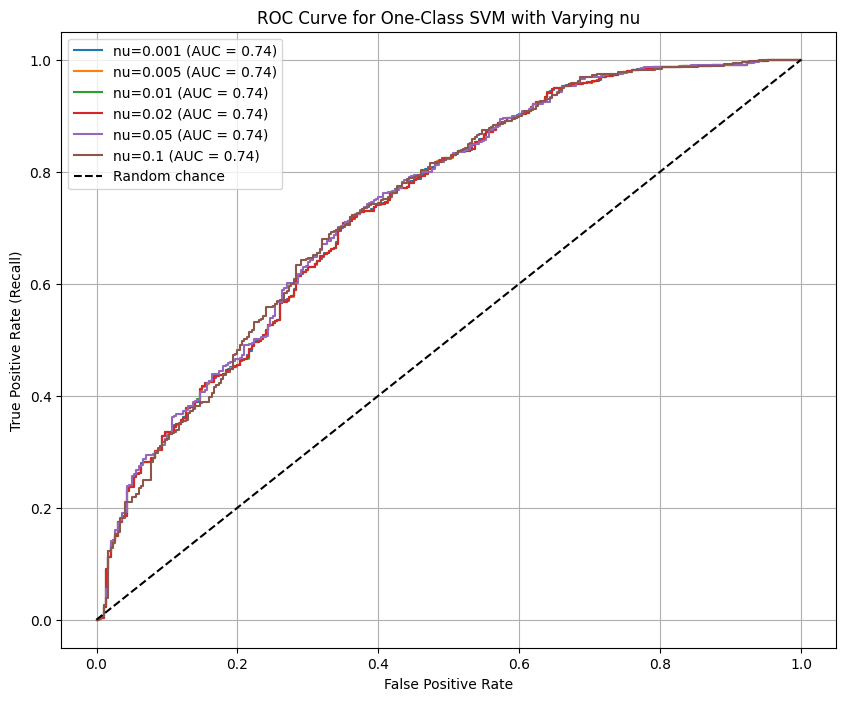
\includegraphics[width=\linewidth]{./Figures/vggish_nu.png}
        \label{fig:image1}
    \end{minipage}
    \hfill
    \begin{minipage}{0.48\textwidth}
        \centering
        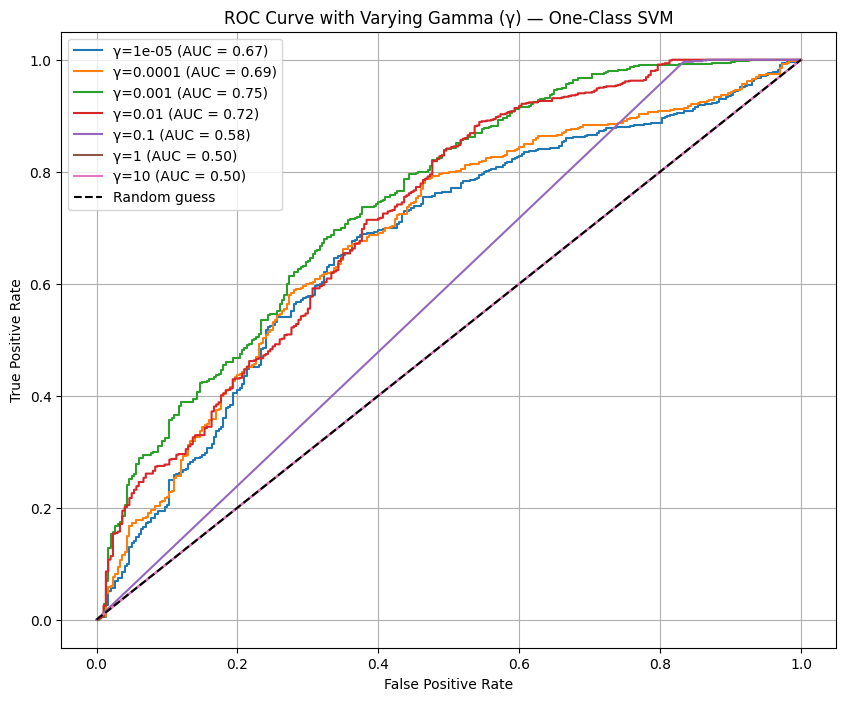
\includegraphics[width=\linewidth]{./Figures/vggish_gamma.png}
        \label{fig:image2}
    \end{minipage}
    \label{fig:side_by_side}
\end{figure}

\section*{Method II: LSTMs for frame prediction}

As a second method, we adopt a different approach. 
Initially, we visualize various samples from the dataset by sampling the audio file with a sample rate of 16k, using a mono channel, to better understand the main differences between anomalous and normal data. 
We represent the audio signals in both the time and frequency domains and highlight the key distinctions between samples from the two groups.
\\Since the representation in the frequency domain alone does not prove meaningful for our task, we decide to proceed by applying a representation on the spectrogram,
 enabling visualization of variations in both time and frequency domains. Figure \ref{fig:spectograms} shows two signals, respectively anomalous and normal. 
 We observe that the anomalous signal is characterized by higher frequencies occurring at intervals defined in the time domain, while the anomalous signal is more regular and stable.

Our method is based on dividing the signal into frames and using an LSTM model to predict the next frame. The strategy can be summarized in the following steps:
\begin{enumerate}
  \item Train an LSTM model on the training data (consisting only of normal data) to learn the normal behavior.
  \item Test the model on an evaluation set, taken from the training data, to assess its performance on unseen normal samples.
  \item Compute the prediction error to define a classification threshold \( T \).
  \item Test the model on the test set and compute the error for each sample. If the sample’s error exceeds \( T \), classify it as anomalous data.
\end{enumerate}


In particular, the spectrogram of each sample is characterized by 313 frames (in the time domain) with 128 features each (each feature corresponds to a frequency value). 
We use a sliding window to define sequences of 10 frames and build the ground truth as the next frame of the spectrogram. 
This results in 303 sequences for each sample, and a total of \(303 \times \text{\#input\_dimension}\) sequences for the training set.
We subsequently train a 2-layer LSTM with an input size of 128 and a hidden size of 256 for 10 epochs, using a learning rate of \texttt{1e-3} and a batch size of 32.

For phase \(2\), the model is evaluated on the evaluation set, and for each sample we compute the average prediction error across all 303 sequences.
Then, we calculate the overall average prediction error and variance across all samples for defining the threshold for classification. \\We test different threshold values, both considering the variance term and ignoring it, and observe the best performance on the test set.

Finally, we plot the ROC curve to determine the best threshold value.
\\Figure \ref{fig:rocLSTM} shows the ROC curve obtained by considering all possible threshold values from the evaluation phase. The final AUC (Area Under the Curve) value is 0.9406, which represents our best result and is close to the optimal case where the AUC is 1.

We also compute the optimal threshold value by selecting the point on the ROC curve closest to the top-left corner, which corresponds to the ideal classifier with a True Positive Rate of 1 and a False Positive Rate of 0. 
This is done by calculating the Euclidean distance between each point \((\text{FPR}, \text{TPR})\) on the curve and the point \((0, 1)\), and choosing the threshold that minimizes this distance. 
The best threshold found is approximately 0.001688, which is close to the mean prediction error observed during the evaluation phase.


As shown in Table \ref{tab:results}, setting the threshold to 0.001688 yields strong performance metrics in terms of precision, recall, and overall F1 score.

\begin{figure}[h]
    \centering
    \includegraphics[width=.5\textwidth]{./Figures/ROC\_LSTM.png}
    \caption{ROC curve for the LSTM model}
    \label{fig:rocLSTM}
\end{figure}

\begin{figure}[h]
    \centering
    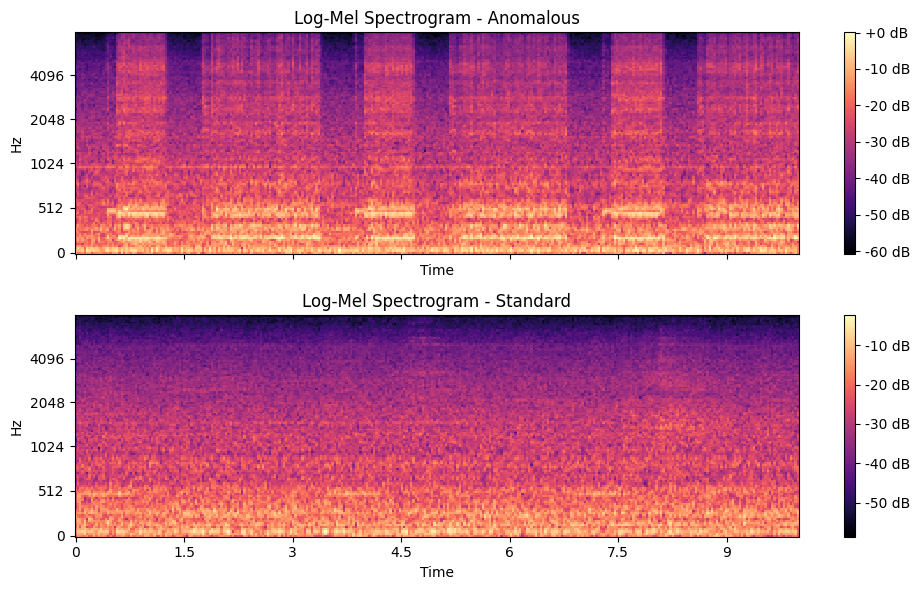
\includegraphics[width=.5\textwidth]{./Figures/spectograms.png}
    \caption{Spectrograms for Anomalous (top) and Normal samples (bottom). As we can observe normal samples are characterized by more stability and lower frequencies.}
    \label{fig:spectograms}
\end{figure}


\begin{table}[h]
    \centering
    \begin{tabular}{|c|c|c|c|}
        \hline
        Class & Precision & Recall & F1-score \\
        \hline
        normal  & 0.76  & 0.90   & 0.82   \\
        anomalous  & 0.96  & 0.89  & 0.92  \\
        \hline
    \end{tabular}
    \caption{Results for LSTM classifier with threshold 0.001688.}
    \label{tab:results}
\end{table}

\section*{Method III: GRU Autoencoder for Sequence Reconstruction}

Our third approach leverages a GRU-based autoencoder to detect anomalies through sequence reconstruction. Unlike the frame prediction strategy in Method II, this method focuses on reconstructing entire input sequences and uses the reconstruction error as an anomaly score. The implementation follows these steps:

\begin{enumerate}
  \item \textbf{Spectrogram Extraction:} As for Method II, convert the audio to log-mel spectrograms (128 mel bands, 16 kHz sampling rate), yielding time-frequency matrices of shape \(T \times 128\) with \(T=313\).
  \item \textbf{Sliding Window Processing:} Generate input sequences using a sliding window of 10 frames (\(T_{\text{seq}} = 10\)), creating \(T - 10\) sequences per sample. Normal training data produces \(303\) sequences per sample on average.
  \item \textbf{Autoencoder Design:} A 2-layer GRU encoder (hidden size 256) compresses sequences into latent states. A symmetric GRU decoder reconstructs the input from these states, followed by a linear layer to match the input dimension (128).
  \item \textbf{Training:} Minimize mean squared error (MSE) between input and reconstructed sequences using Adam (\(\text{lr} = 10^{-3}\), batch size 64) for 10 epochs.
  \item \textbf{Threshold Calibration:} Plot the ROC curve for the training set to determine the optimal threshold. In this case a TPR of 0.8 is chosen, corresponding to a FPR of 0.123. The resulting threshold is \(\tau = 0.000511\).
  \item \textbf{Inference:} For test samples, average the MSE across all sequences. Classify samples as anomalous if their average MSE exceeds \(T\).
\end{enumerate}

\noindent The model achieves a validation MSE of \(0.000484 \pm 0.000050\), indicating stable reconstruction of normal patterns. On the test set, it attains an AUC of \(0.892\), with precision-recall trade-offs shown in Table~\ref{tab:gru_results}. The ROC curve (Figure~\ref{fig:rocGRU}) visualizes that the chosen threshold \(\tau\) effectively balances false positives and true positives (FPR = 12.3\%, TPR = 80.0\%).
\begin{figure}[h]
    \centering
    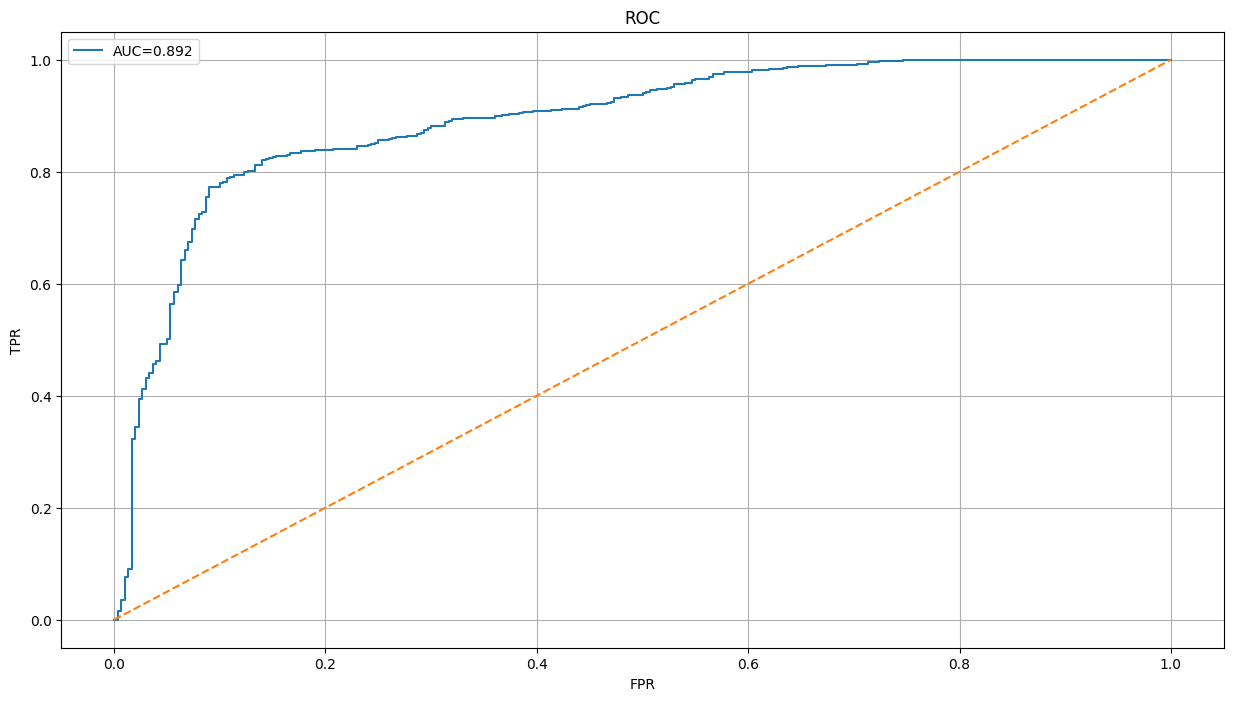
\includegraphics[width=\textwidth]{./Figures/ROC_Autoenc.png}
    \caption{ROC curve for the GRU autoencoder (AUC = 0.892). The red marker indicates the 90th-percentile threshold.}
    \label{fig:rocGRU}
\end{figure}
\noindent The GRU autoencoder's performance is summarized in Table~\ref{tab:gru_results}. The model achieves a precision of 0.94 and a recall of 0.80 for the anomalous class, indicating its ability to identify anomalies effectively. However, the precision for the normal class is lower at 0.62, suggesting that some normal samples are misclassified as anomalies.
\begin{table}[H]
    \centering
    \begin{tabular}{lccc}
        \toprule
        Class & Precision & Recall & F1-score \\
        \midrule
        Normal & 0.62 & 0.87 & 0.72 \\
        Anomaly & 0.94 & 0.80 & 0.87 \\
        \bottomrule
    \end{tabular}
    \caption{Performance of the GRU autoencoder at \(T = 0.000511\).}
    \label{tab:gru_results}
\end{table}
\noindent While this method simplifies anomaly detection to a reconstruction task, its performance lags slightly behind Method II's LSTM predictor.%, likely due to the autoencoder's tendency to "memorize" normal patterns rather than learn temporally sensitive transitions. Hybrid architectures combining prediction and reconstruction objectives could mitigate this limitation.

\section*{Conclusion}

This project addresses Anomalous Sound Detection (ASD) for a "Slide Rail" machine, training models exclusively on normal operational sounds to replicate DCASE challenge conditions. We explore three methods: \textbf{VGGish} embeddings with\textbf{ One-Class SVM}, an \textbf{LSTM} for next-frame prediction on spectrograms, and a \textbf{GRU-based autoencoder} for sequence reconstruction.

Comparative evaluation reveal that the\textbf{ LSTM-based} frame prediction model (Method II) delivers the strongest performance. It achieves a superior Area Under the \textbf{ROC Curve} (AUC) of \textbf{0.9406} and an \textbf{F1-score} of\textbf{ 0.92} for detecting anomalies.\\
This indicates that modeling temporal sequences in spectrograms via LSTMs is more effective for identifying deviations from normal machine operation than the feature-based SVM or the GRU autoencoder's reconstruction approach for this dataset. The LSTM's ability to capture normal sound patterns and flag deviations proves most successful in this type of task.

\end{document}
